\documentclass[12pt]{article}

\usepackage{subfigure}
\usepackage{pstricks}
\usepackage{pst-node}
\usepackage{graphicx}
\usepackage{authoraftertitle}
\usepackage[T1]{fontenc}
\usepackage{amsmath}
\usepackage{amsfonts}
\usepackage{amssymb}
\usepackage{algorithm2e}
\usepackage{xspace,epsfig,url}
\usepackage{pst-plot,pstricks-add}

\newtheorem{theorem}{Theorem}
\newtheorem{definition}[theorem]{Definition}
%\newtheorem{remark}[theorem]{Remark}

\newenvironment{remark}
{% This is the begin code
\stepcounter{theorem}\vspace*{0.3cm}\noindent{\bf Remark} \arabic{theorem}.
}
{% This is the end code
}

\newtheorem{proposition}{Proposition}[section]
%\newtheorem{cor}[thm]{Corollary}

\newcommand{\comment}[2]{{\color{red}{\bf (#1: #2)}}}
\newcommand{\greedyAlgo}{\textsc{Greedy}}


\linespread{1.5}

\setlength{\leftmargin}{3.5cm}

\setlength{\topmargin}{2cm}

\setlength{\rightmargin}{2cm}

\newcommand{\ics}[2]{\langle #1, #2 \rangle}
%\newcommand{\ics}[2]{\frac{#1}{#2}}

\title{Algorithmic Optimization and Parallelization of Eppstein's Synchronizing Heuristic}

\author{Serta\c{c} Karahoda}

\date{}

\begin{document}

\maketitle
\thispagestyle{empty}
\vspace{1cm}

\begin{center}
Submitted to the Graduate School of Sabanc{\i} University \\
in partial fulfillment of the requirements for the degree of \\
Master of Science
\end{center}

\vspace{2cm}

\begin{center}
Sabanci University
\end{center}

\begin{center}
Augustus, 2017
\end{center}


\newpage
$ $
\thispagestyle{empty}
\newpage
$ $
\vspace{5cm}
\begin{center}
\copyright \hspace{0.1cm} \MyAuthor\space 2015

All Rights Reserved
\thispagestyle{empty}
\end{center}
\newpage

\begin{center}
\large
\MyTitle
\end{center}

\begin{center}
\MyAuthor

CS, Master's Thesis, 2017

Thesis Supervisor: H\"{u}sn\"{u} Yenig\"{u}n\\
Thesis Co--Supervisor: Kamer Kaya
\end{center}

\begin{center}
Keywords: ...
\end{center}

\begin{abstract}
...
\end{abstract}
\newpage

\begin{center}
\large
Eppstein'\i{}n S\i{}f\i{}rlama Sezgiselinin Algoritmik Eniyilemesi ve Paralelle\c{s}tirilmesi
\end{center}

\begin{center}
\MyAuthor

CS, Y\"{u}ksek Lisans Tezi, 2017

Tez Dan{\i}\c{s}man{\i}: H\"{u}sn\"{u} Yenig\"{u}n\\
Tez E\c{s}dan{\i}\c{s}man{\i}: Kamer Kaya
\end{center}

\begin{center}
Anahtar Kelimeler: ...
\end{center}

\begin{quote}
\begin{center}
{\bf \"{O}zet}
\end{center}

...

\end{quote}
\newpage
$ $
\vspace{2cm}
\begin{center}
\textbf{Acknowledgements}
\end{center}

%I would like to state my gratitude to my supervisor, H\"{u}sn\"{u} Yenig\"{u}n for everything he has done for me, especially for his invaluable guidance, limitless support and understanding. \\
%I would like to thank Hasan Ural and Guy-Vincent Jourdan for supporting this work with precious ideas and comments. \\
%I would like to thank my family for never leaving me alone. \\
%The financial support of Sabanci University is gratefully acknowledged. \\
%I would like to thank TUBITAK for the financial support provided.


\newpage
\tableofcontents

\newpage 
\listoffigures

\newpage
\listoftables



\newpage
\section{Introduction}
\label{sec:Intro}

\comment{Sertac}{Reset word'den bahsedecegim.}

\comment{Sertac}{Intro'da FSM'den bahsedecegim.}

\newpage
\section{Preliminaries}
\label{sec:Preliminaries}
FSMs are mathematical abstractions for of real word systems. When an FSM gets an input, it moves from a state to another with an output. Since synchronization sequence consider only destination state, the output is not in the scope of this work. Therefore, we can consider FSMs are as automata with simple transaction function without an output.

When an {\em automaton} is complete and deterministic, it is defined by a triple $A=(S, \Sigma, \delta)$  where $S = \{1, 2, \ldots, n\}$ is a finite set of $n$ states, $\Sigma$ is a finite alphabet consisting of $p$ input symbols (or simply {\em letters}). $\delta : S \times \Sigma \rightarrow S$ is a transition function. If the automaton $A$ is at a state $s$ and if an input $x$ is applied, then $A$ moves to the state $\delta(s,x)$. Figure~\ref{fig:inv} shows an example automaton $A$ with 4 states and 2 inputs using graphical notation.\looseness=-1

\begin{figure}[h]
\centering
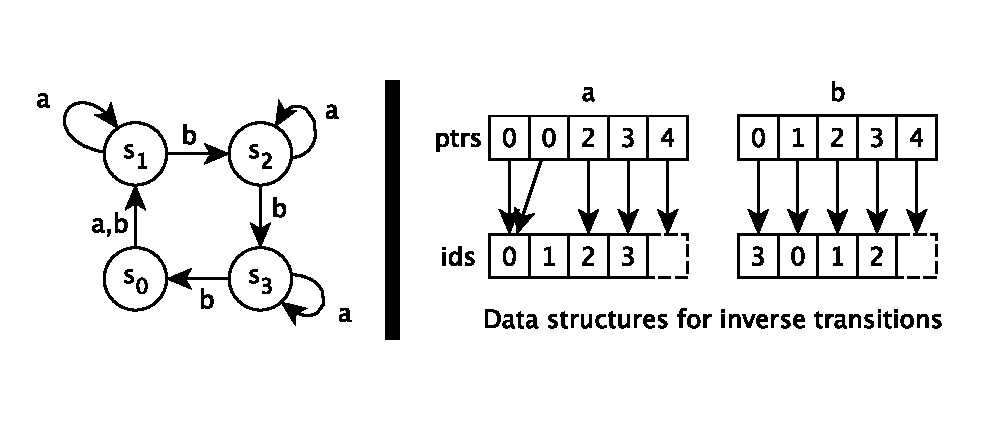
\includegraphics[width=0.7\textwidth]{figs/inverse.pdf}
\caption{A synchronizable automaton $A$~(left), and the data structures we used to store and process
the transition function $\delta^{-1}$  in memory (see Section~\ref{subsec:imp} for the details). A synchronizing sequence for $A$ is $abbbabbba$. \comment{sertac}{caption cok uzun belki iki figure olarak ayri ayri anlatabiliriz}}
\label{fig:inv}
\vspace*{-3ex}
\end{figure}

An element of the set $\Sigma^\star$ is called an {\em input sequence} (or simply {\em word}). $|w|$ denotes the length of $w$, and $\varepsilon$ expresses the empty word. Transition function $\delta$ can be extended to a set of states and to a word in the usual way. With fact $\delta(s,\varepsilon)=s$, let a word $w \in \Sigma^\star$ and a letter $x \in \Sigma$, then $\delta(s,xw) = \delta(\delta(s,x),w)$. Likewise, for a set of states $S' \subseteq S$, transaction function is $\delta(S',w) = \{ \delta(s,w) | s \in S'\}$.

Inverse of the transaction is also a well defined function. $\delta^{-1}(s,x)$ denotes the set of those states with a transition to state $s$ with input $x$. Formally, $\delta^{-1}(s,x) = \{ s' \in S | \delta(s',x)= s\}$.

Let $A=(S, \Sigma, \delta)$ and $S^{\langle 2 \rangle} = \{ \langle s_i, s_j \rangle | s_i,s_j \in S \}$ be set of multisets  with cardinality 2. For $\langle s_i, s_j \rangle \in S^{\langle 2 \rangle}$, if $s_i=s_j$ then it is called as \textit{singleton}, otherwise called as \textit{pair}. 

Let $C \subseteq S$ and $w \in \Sigma^*$, when cardinality of $\delta(C,w)$ is 1 then $w$ is \textit{merging sequence} for $C$. If $C=S$, $w$ is called \textit{reset word} of automaton.




\newpage
\bibliographystyle{plain}
\bibliography{thesis}

\end{document}


